\renewcommand\thetable{\arabic{chapter}-\arabic{table}}
%\renewcommand\thefigure{\arabic{chapter}-\arabic{figure}} 
\chapter{校舍資訊與破壞構件之關係模型}

校舍耐震評估最準確的階段為進行詳細評估作業,但進行校舍詳細評估須歷經非常多之流程如圖~\ref{fig:FLOW}~,花費很多時間,如能有一輔助工具在校舍詳細評估前期即可粗估校舍之可能破壞構件與其破壞模式,將有助於技師與專業人是進行作業時先有初步結果之掌握,瞭解校舍的弱點以及可能的破壞形式,便能夠針對這些重點多加檢視,提升整體之評估水準,因此本研究也對於此一知識進行探勘分析。

在校舍耐震資料庫中所記錄的校舍破壞元件的資訊,是記錄在\nameref*{appendix-de}中之資訊,記錄了校舍在詳細評估的側推分析下,首先破壞的結構元件,包括了樑、柱、窗台柱、磚牆、RC~牆等構件,並且記錄了破壞樓層以及破壞形式,如剪力破壞、撓曲破壞等。而本分析之目標則是要尋找此一資料集與校舍的基礎設計參數間之關係,而由於要分析的破壞構件種類較多,難以用單一個模型建構出其多重關係,因此本分析將此問題拆成數個較為單純的問題,單獨針對不同構件是否破壞進行資料探勘分析,並將主要的正向破壞挑出作為探勘目標,分別進行了五組資料探勘分析。


\section{資料前處理}

本分析之前處理分為三個階段,分別為資料合理性篩選、資料屬性的篩選以及新屬性之合成,首先,資料之合理性分析一樣依照~NCREE~所建議之規則篩選,資料屬性之挑選則分為兩個步驟,第一個步驟是根據資料之分佈挑選資料子集合,藉由此一步驟可以適當的排除少數結構形式的校舍,並同時縮減資料屬性的數量,降低資料複雜度,挑選的條件為:

\begin{itemize}
\item 鋼筋混凝土建築
\item 單邊走廊且廊外無柱
\item 無地下室
\end{itemize}

同時由於選出資料的此三屬性的數值均相同,因此死此三個條件相關的屬系便在此過程被過剔除;接著則是進一步挑選資料屬性,降低資料的複雜度,本分析依照不同屬性與校舍耐震能力間之關係作為挑選依據,將完全無關以及有重複性質之屬性剔除,再將重要性較高之屬性挑選出,並保持屬性數量不要過多,並根據測試結果合成出部分新屬性,最後挑選之屬性如下:

\begin{multicols}{2}
\begin{itemize}
\item 校舍長度
\item 校舍深度
\item 樓層數
\item 地上層樓地板總面積
\item 一樓教室柱根數
\item 一樓走廊外柱斷面積和
\item 475~年設計地表加速度
\item 校舍垮距
\item 用途係數
\item X~向~1F~三面圍束磚牆斷面積
\item 有無三面圍束磚牆
\item 有無四面圍束磚牆
\item 有無磚牆
\item 同時有三面和四面圍束磚牆
\item 有無~RC~牆
\item[]
\end{itemize}
\end{multicols}

其中校舍跨距資料是根據現有資料推估的估計值,因此一資料並未在校舍補強工作的流程當中有紀錄,合成之公式為:

\begin{equation} \dfrac{\text{校舍長度}}{^{\text{一樓教室柱根數}}/_2 - 1} \label{eq:span}\end{equation} 

本分析其餘所挑選之資料屬性介紹與選擇說明如下:

\begin{description}
  \item[校舍長度、深度]
  中小學校舍中之典型校舍其建築形式較為固定且普遍存有耐震能力較弱之現象,因此本分析推測在這些典型校舍中,某些特定尺寸之校舍應與其極限強度下會破壞之構件與其破壞模式存有一定之相關性。因此本分析將此二屬性納入屬性集做為本探勘模型之輸入屬性。
  \item[樓層數]
  加入此屬性,其構想為假設這些校舍中應該有集中幾層樓之建築與其極限強度下會破壞之構件與其破壞模式存有一定之相關性。因此本分析將此屬性納入屬性集做為本探勘模型之輸入屬性。希望藉由其中隱藏之關聯性達到目標之預測。
  \item[地上層樓地板總面積]
  校舍之樓地板面積亦屬於建築形式之一環,因此可視為該校舍之特有形式,本分析假設在典型校舍中存有特定樓地板面積大小有其普遍對應之耐震能力或某些尺寸之樓地板面積可能存有接受補強較高的機率。
  \item[一樓教室柱根數]
  教室柱之根數間接可之校舍樓地板面積之大小或規模,因此本分析將之視為影響工程經費之因素之一,經將此屬性納入探勘模型中測試後,也確實發現此屬性對預測之正確率有一定之提升。
  \item[一樓走廊外柱斷面積和]
  台灣中小學校舍其建築形式較為固定,教室柱之多寡或其尺寸亦可視為建築形式中之一環,因此本分析推測在這些校舍中,教室柱應該存有某些特定總斷面積大小之校舍其耐震能力較差,因此本分析將此屬性納入屬性集做為本探勘模型之輸入屬性。
  \item[475~年設計地表加速度]
  由校舍所在位於查出其工址短週期設計水平譜加速度之~0.4~倍($0.4S_{DS}$),同時也代表耐震需求,是判斷耐震能力是否足夠非常重要的屬性。
  \item[用途係數]
  該屬性為紀錄該校舍是否作為緊急避難使用,以決定其值為~1.25~或~1.5~,為反映其因重要性所需之安全係數。如該校舍當初規劃為緊急避難使用,那其當初設計強度就會比較高,用途係數除了可以反應校舍耐震能力之需求外,校舍最初在設計建造時,校舍對於耐震能力需求的差異,應該也會直接反映在校舍實際的耐震能力上,因此將之加入本屬性集內。
  \item[X~向一樓三面圍束磚牆總斷面積]
  磚牆對校舍能提供部分耐震能力,本分析試過單獨放入三面圍束、四面圍束與同時放入三面與四面圍束磚牆,經分別試驗不同之屬性集,建立多個不同的模型,其結果以單獨使用三面圍束磚牆總斷面積做為輸入屬性,其預測之結果最佳。
  \item[有無三面圍束磚牆]
  此屬性為校舍資料庫不存在之欄位,因經測試許多屬性集與不同探勘方法發現磚牆對預測結果有一定影響力,但並不是所有校舍均有磚牆,為利用此一資訊,將資料中紀錄有無三面圍束磚牆之屬性作為依據,當該值表示該校舍有三面圍束磚牆時,此屬性值為~1~,反之則為~0~。
  \item[有無四面圍束磚牆]
  此屬性為校舍資料庫不存在之欄位,因經測試許多屬性集與不同探勘方法發現磚牆對預測結果有一定影響力,但並不是所有校舍均有磚牆尤其是四面圍束磚牆,為利用此一資訊,將資料中紀錄有無四面圍束磚牆之屬性作為依據,當該值表示該校舍有四面圍束磚牆時,此屬性值為~1~,反之則為~0~。
  \item[有無磚牆]
  此屬性為校舍資料庫不存在之欄位,因經測試許多屬性集與不同探勘方法發現磚牆對預測結果有一定影響力,但並不是所有校舍均有磚牆,因此本分析建立此一屬性單純記錄校舍是否有磚牆,如果校舍有磚牆則值為~1~,反之則為~0~。
  \item[同時有無三面和四面圍束磚牆]
  此屬性也為校舍資料庫不存在之欄位,因經測試許多屬性集與不同探勘方法發現磚牆對預測結果有一定影響力,且進一步測試發現校舍是否同時存有三面圍束與四面圍束磚牆對其預測結果,存有一定影響力。因此本分析變希望因此本分析為利用此一資訊總和上面所介紹之\textbf{有無三面圍束磚牆}及\textbf{有無四面圍束磚牆}之資訊合成出此一屬性,如果校舍同時有三面圍束和四面圍束磚牆,此屬性之值為~1~,反之則為~0~。\\
  以上四欄位之組合即隱含校舍結構物之磚牆類型組合資訊。
  \item[有無~RC~牆]
  此屬性為校舍資料庫不存在之欄位,因經測試許多屬性集與不同探勘方法發現~RC~對預測結果有一定影響力,但並不是所有校舍均有~RC~牆,因此本分析單獨建立亦屬性只記錄該校舍是否有~RC~牆,如果有~RC~牆,則值為~1~,反之則為~0~。
\end{description}

前處理完成後共有~297~筆資料,並且每筆資料有~15~個資料屬性,其中有~139~棟校舍的樑有破壞,227~棟校舍有柱破壞,228~棟校舍有窗台柱破壞,11~棟校舍有~RC~強破壞,175~棟校舍有磚牆破壞。

\section{資料探勘與結果}

由於校舍之構件種類眾多,破壞構件的種類組合也變的複雜許多,以本資料庫中有紀錄到的五種構件來說,每棟校舍的構件是否有破壞的組合就有~32~種,因此本研究把原本輸出結構複雜之模型分為數個較單純的模型來探勘,每種構件單獨探勘尋找出其是否會破壞與校舍基礎設計參數間之關係模型,而構件是否破壞這個屬性為布林值(Boolean),輸出目標為布林值之模型,其知識的型態可以歸類到資料探勘中的分類形式,而支撐向量機在分類探勘上之表現良好,運算速度也很快,因此本分析採用此探勘方法,依據前處理完之~297~筆資料並挑選屬性集內之欄位,將整體資料分為訓練集與測試集,比例為訓練集~70\%~、測試集~30\%~,以此做為探勘此關係模型之方法,評斷模型優劣的指標則為關係模型之正確率,重複分析並調整參數到穩定,其中,除柱破壞模型之~kernel~為~RBF(radial basis function)~外,其餘構件之破壞關係模型所選擇之~kernel~均為~polynomial,兩者均為~SVM~常使用的~kernel type~,RBF~之特色是它代表了不同筆資料間之相似程度,而~polynomial
~則是除了各個輸入屬性的特性之外,還同時包含了不同屬性組合時之特性。SVM~之參數挑選為~$\epsilon$~為~$0.1$~、誤差之懲罰值~$C$~為~$10$,使用~RBF kernel~時之~$\gamma$~為~$0.1$、收斂條件則為~$0.001$,SPSS Clemitine~之節點架構如圖~\ref{fig:crack-flow}~所示,在此設定下所產出之模型結果如表~\ref{tab:comp_result}。

\begin{figure}[hbtp]
  \begin{center}
    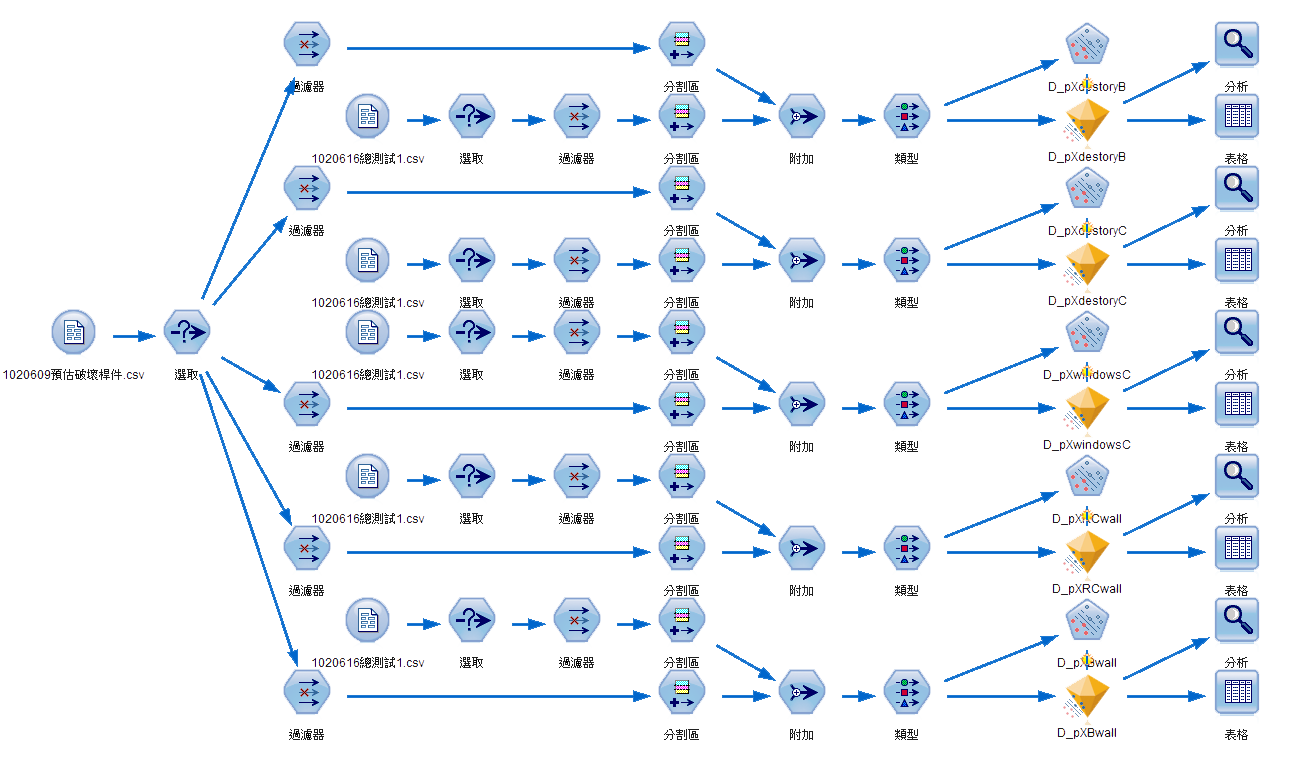
\includegraphics[width=1.0\textwidth]{figures/crack-flow.png}
    \caption{構件破壞模型探勘流程} 
    \label{fig:crack-flow}
  \end{center}
\end{figure}


\setlength{\tabcolsep}{2em}
{\renewcommand{\arraystretch}{1.5}
\begin{table}[hbtp]
  \begin{center}
    \caption{破壞構件關係模型結果}
    \label{tab:comp_result}
    \begin{tabular}{l c c}
    	\hline
    	破壞元件 & 資料集 & 正確率 \\
    	\hline
    	\multirow{2}{*}{X 正向樑破壞} & 訓練集 & 76.97\% \\
    	\cline{2-3} & 測試集 & 82.14\% \\
    	\hline
    	\multirow{2}{*}{X 正向柱破壞} & 訓練集 & 86.52\% \\
    	\cline{2-3} & 測試集 & 86.90\% \\
    	\hline
    	\multirow{2}{*}{X 正向窗台柱破壞} & 訓練集 & 79.21\% \\
    	\cline{2-3} & 測試集 & 77.38\% \\
    	\hline
    	\multirow{2}{*}{X 正向~RC~牆破壞} & 訓練集 & 99.32\% \\
    	\cline{2-3} & 測試集 & 98.25\% \\
    	\hline
    	\multirow{2}{*}{X 正向磚牆破壞} & 訓練集 & 80.34\% \\
    	\cline{2-3} & 測試集 & 80.95\% \\
    	\hline
    \end{tabular}
  \end{center}
\end{table}
}


根據表~\ref{tab:comp_result}~所示,可以發現五種構件的破壞關係模型的表現均不錯,正確率都有超過~75\%~,甚至~80\%~,其中~RC~牆的部分正確率特別高,其原因是校舍中有~RC~牆的校舍比例偏低,因此關係模型在訓練時會找到校舍是否有~RC~牆和是否有~RC~牆破壞的高度關聯性,因此沒有~RC~牆的校舍都很容易就判斷為沒有~RC~牆破壞,實際上在~297~棟校舍當中,只有~39~棟校舍有~RC~牆,如果只看這~39~棟校舍,則正確率有~89.7\%,且沒有~RC~牆的校舍當中,只有一棟校舍判斷錯誤。

%本探勘模型使用支援向量機並分別針對耐震詳細評估資料表之性能點狀態下最嚴重破壞樓層之主要破壞桿件及其破壞模式進行預測,其各項之預測正確率如下: \\ \indent
%X~正向樑破壞 97.06\% \\ \indent
%X~正向柱破壞 100\% \\ \indent
%X~正向窗台柱破壞 94.12\% \\ \indent
%X~正向 RC 牆破壞 100\% \\ \indent
%X~正向磚牆破壞 82.6\% \\ \indent


%beam, 139
%  train  5/262
%  test   1/34

%column, 227
%  train  36/262
%  test   0/34

%window, 228
%  train  2/262
%  test   2/34

%rc wall, 13
%  train  5/262
%  test   0/34

%brick wall, 175
%  train  48/262
%  test   5/34

% 最後並根據每棟校舍於性能點狀態下,各項破壞構件其破壞模式進 行正確率之計算,根據耐震詳細評估資料表內有五項破壞構件之欄位,因此本分析假設該校舍於每項破壞構件之欄位如預測正確,則加正確率百分之二十,共五項欄位,如各項接預測正確,則該校舍針對其性能點狀態下最嚴重破壞樓層之主要破壞桿件及其破壞模式之預測正確率為百分之百。其 34 棟總體校舍針對 5 種破壞構件及其破壞模式之平均預測正確率為 95.3\%。本預測目標其欄位屬性為類別型態,因此無法以其他評估指標進行比較,一般評估指標只能用來評估數值型資料。34 棟校舍於破壞構件及其破壞模式之預測資料與結果如,X 正向樑破壞於表 5.6 中欄位名稱為 D\_pXdestoryB,X 正向柱破壞於表 5.6 中欄位名稱為~D\_pXdestoryC,X 正向窗台柱破壞於表 5.6 中欄位名稱為 D\_pXwindowsC,X 正向 RC 牆破壞於表 5.6 中欄位名稱為 D\_pXRCwall,X 正向磚牆破壞於表 5.6 中欄位名稱為 D\_pXBwall,其餘之欄位說明如表 5.5。
